\documentclass[10pt]{article}
\usepackage[margin=1.6cm]{geometry}
\usepackage{graphicx}
\usepackage{amsmath}
\usepackage{amssymb}
\usepackage{booktabs}
\usepackage{float}
\usepackage[hidelinks]{hyperref}
\setlength{\parskip}{2pt}\setlength{\parindent}{0pt}

\title{\vspace{-1.4cm}Rescuing a trained singleton solution by planting a degree-4 circuit:\\
a finite seed barrier at $\rho_{\rm crit}\approx0.283$\\
\large one-hidden-layer ReLU net, $d=8$, inputs $x_1..x_8$ and $p=x_1x_2x_3x_4$, $q=x_5x_6x_7x_8$, target $\chi_8=pq$}
\author{}\date{\vspace{-1.2cm}}

\begin{document}\maketitle\vspace{-1.7cm}

\section*{Setup}
\textbf{Source model.} The final checkpoint of \texttt{rank1\_d8\_s44\_nobn\_wd1e-2\_Q8.0\_50k}
(sha256 \texttt{41849d5c\ldots}, step 50\,000): $y(x)=r^{\top}\mathrm{ReLU}(WV^{\top}\phi(x))$ with
$V\in\mathbb R^{10\times1024}$ (eight singleton rows initialised $8\times$ larger than the two degree-4
rows), $W\in\mathbb R^{1024\times1024}$, $r\in\mathbb R^{1024}$, no biases, no bottleneck; SGD, lr
$10^{-3}$, momentum $0.9$, batch 512, weight decay $\lambda=0.01$ on $V,W,r$. On the full cube it is a
pure singleton solution: MSE $5.0\cdot10^{-3}$, objective $\mathcal L=\mathrm{MSE}+\tfrac\lambda2\sum\|\theta\|^2
=0.2023$ (prediction $0.20196$), target coefficient $a=0.929$, degree-4 pre-activation share $10^{-7}$.
Every unit is a sign template $z_j\propto\sum_i s_{ji}x_i$.

\textbf{Intervention.} $M=4$ silent units $J=\{195,404,471,872\}$ (output RMS $1.4\cdot10^{-8}$) and two
directions $U=[u_1,u_2]$ orthonormal and orthogonal to every row of $V_0$ (to $6\cdot10^{-17}$). Prepared
baseline $W_{\rm base}=W_0(I-UU^{\top})$, $W_{\rm base}[J]=0$, $r_{\rm base}[J]=0$ (all other
pre-activations preserved to $8\cdot10^{-16}$, penalty change $-1.3\cdot10^{-6}$). Seed of strength $\rho$:
\[
V_p=V_{0,p}+\tfrac{\rho}{\sqrt2}u_1^{\top},\quad V_q=V_{0,q}+\tfrac{\rho}{\sqrt2}u_2^{\top},\quad
W_j=\tfrac{\rho}{\sqrt{2M}}(s_{j1}u_1+s_{j2}u_2)^{\top},\quad r_j=\tfrac{\rho}{\sqrt M}s_{j1}s_{j2},
\]
with $S$ the balanced $\pm1$ pattern matrix, so that exactly $y_\rho-y_{\rm base}=\tfrac{\rho^3}{4}\chi_8$
and $\Delta P=\tfrac{3\lambda}{2}\rho^2$. Validated on all 256 inputs in float64 (errors $\le10^{-15}$) and
float32 (output $5\cdot10^{-7}$, $\Delta\mathcal L$ $3\cdot10^{-12}$); no other Walsh coefficient is
injected; the projections of the negative full-cube regularised gradient onto the three templates equal
$2e\kappa_2\rho^2-\lambda\rho$ ($\kappa_2=\tfrac14$) to $10^{-17}$. Controls: the unmodified checkpoint,
the prepared baseline ($\rho=0$), and \emph{target-orthogonal} seeds (same $V,W$ seed, readout template
replaced by a random unit vector $\perp t_r$: same norm, injected target coefficient $10^{-17}$).

\textbf{Training.} Every arm restarts from an independent copy with a fresh SGD optimiser (zero momentum
buffers; momentum, lr, $\lambda$, batch unchanged), the same minibatch sequence (data seed 777; repeats
778, 779), 50\,000 post-intervention steps; exact full-cube diagnostics every 5 steps to 500, every 100
to 5\,000, then every 250. Unresolved arms were continued to 150\,000 steps (recorded budget). Nothing is
projected, frozen or re-balanced after the intervention. Arms live in
\texttt{runs/plantd4\_Q8\_<arm>\_s<seed>/} (\texttt{analysis/}: metadata, validation, trajectory, final
ablations), continuations in \texttt{runs/plantd4\_Q8L\_*}.

\section*{Results}
\begin{figure}[H]\centering
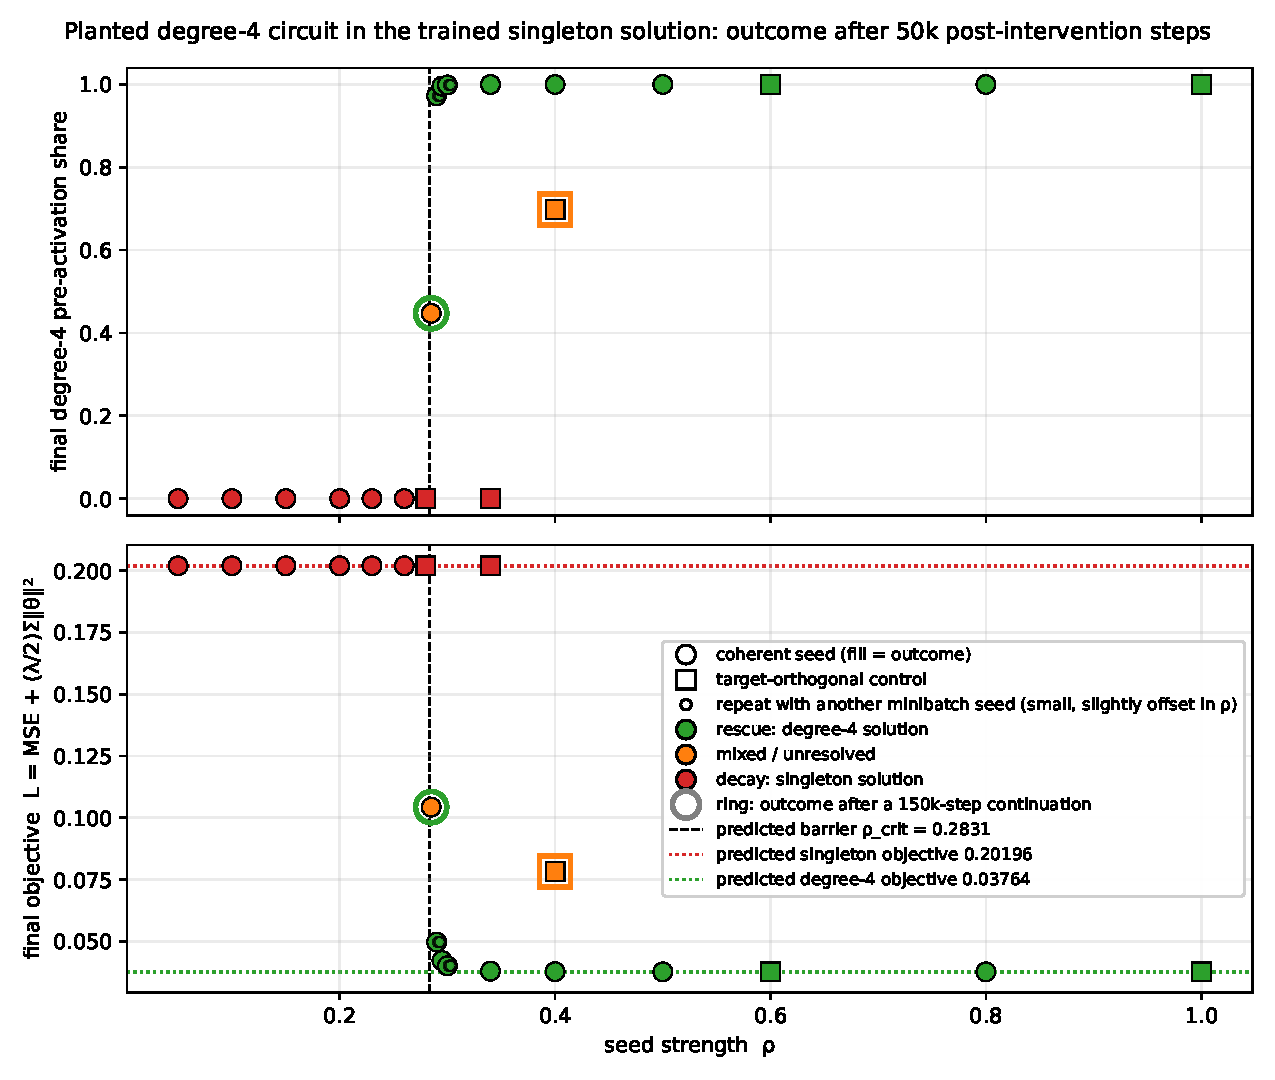
\includegraphics[width=0.54\textwidth]{rank1_bottleneck/plantd4_Q8_summary.pdf}\vspace{-4pt}
\caption{Coarse grid, $\rho\in[0.05,1]$: final degree-4 share (top) and objective (bottom) after 50k
post-intervention steps versus seed strength $\rho$. Fill colour = outcome; small markers = repeats with
other minibatch seeds; rings = outcome after a 150k continuation; squares = target-orthogonal controls.
Dashed line: predicted $\rho_{\rm crit}=0.2831$; dotted lines: predicted limiting objectives $0.20196$
(singleton) and $0.03764$ (degree-4).}
\label{fig:summary}
\end{figure}


\textbf{1. A finite seed barrier exists, at the predicted location.} All coherent seeds with
$\rho\le0.28$ decay back to the singleton solution (three minibatch seeds at $0.28$ agree to four digits),
and all seeds with $\rho\ge0.285$ are rescued: $\rho=0.285$ is mid-takeover at 50k (share $0.45$) and
complete by 75k; $\rho\ge0.29$ complete within 50k. The barrier lies in $(0.280,0.285)$, within $1\%$ of
$\rho_{\rm crit}=0.2831$. On the coarse grid the picture is binary: every seed with $\rho\in\{0.05,0.10,0.15,0.20,0.23,0.26,0.28\}$ decays to $\mathcal L=0.2020$, every seed with $\rho\in\{0.285,\ldots,0.40,0.50,0.60,0.80,1.0\}$ is rescued to the same $\mathcal L=0.0377$ and share $1.000$; a seed $3.5\times$ above threshold ends in exactly the same state as one $1\%$ above it, only faster (takeover complete by 20k at $\rho=0.40$, 40k at $0.30$, 75k at $0.285$).

\textbf{2. Limiting objectives match.} Decayed arms end at $\mathcal L=0.2020$--$0.2022$ (prediction
$0.20196$); fully rescued arms at $0.0376$--$0.0380$ (prediction $0.03764$), with the rest-of-network
target coefficient $\le0.003$ and singleton embedding rows decayed to $\le0.03$. Final ablations confirm the
support: rescued models keep MSE $1.6\cdot10^{-4}$ with the degree-4 inputs alone and lose everything
(MSE $1.0$) with singletons alone; decayed models the reverse.

\begin{figure}[H]\centering
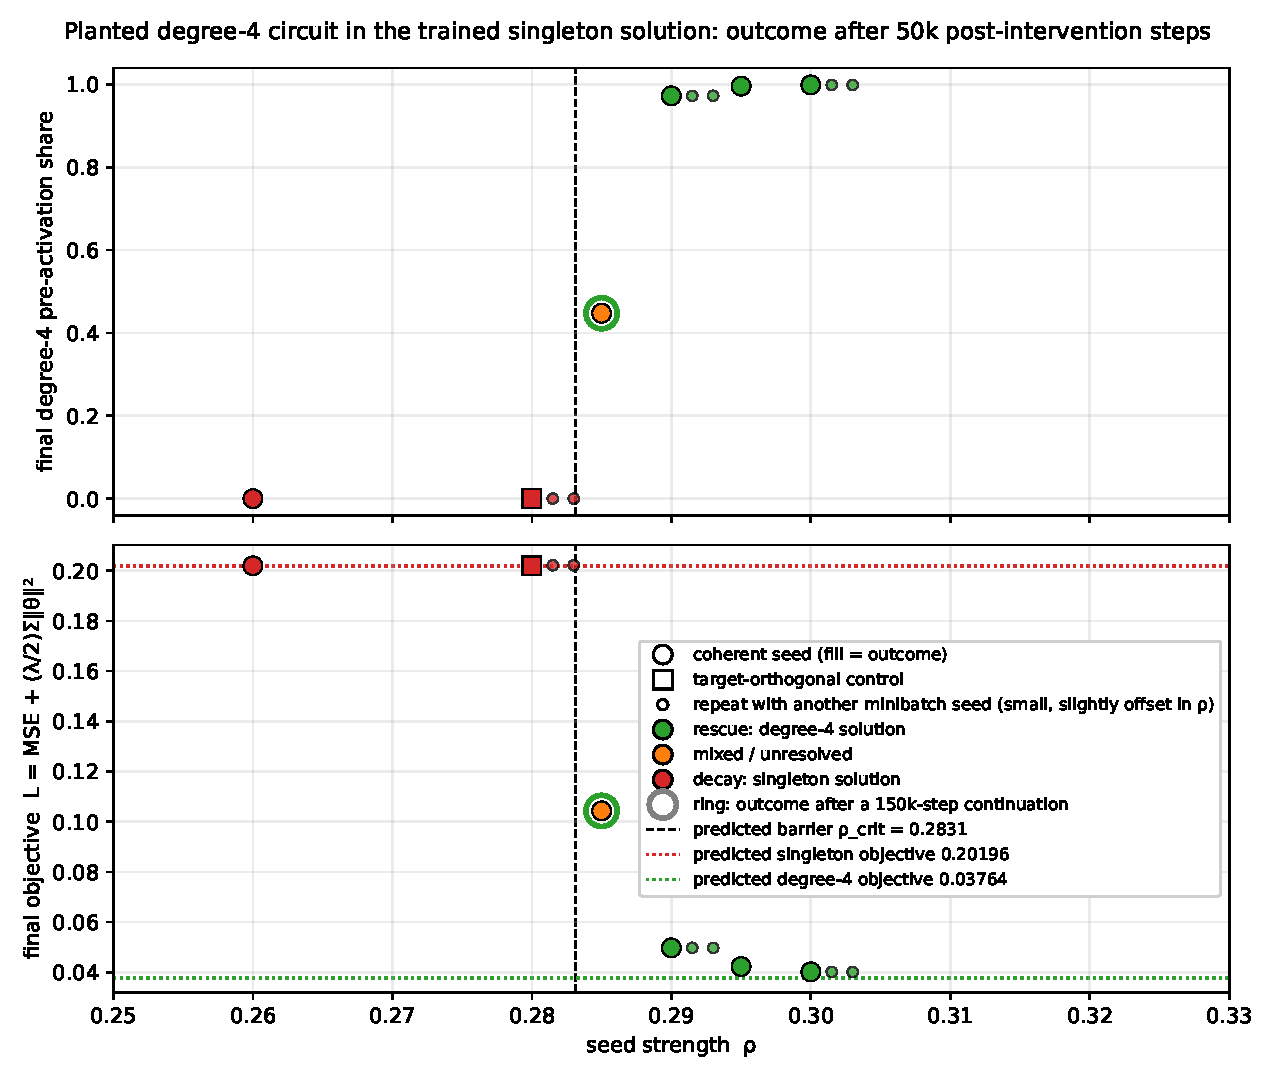
\includegraphics[width=0.54\textwidth]{rank1_bottleneck/plantd4_Q8_summary_zoom.pdf}\vspace{-4pt}
\caption{Zoom of Fig.~\ref{fig:summary} on $\rho\in[0.25,0.33]$, same conventions. The barrier lies between
$\rho=0.28$ (decay, three minibatch seeds) and $0.285$ (rescue after a 150k continuation).}
\label{fig:zoom}
\end{figure}

\begin{figure}[H]\centering
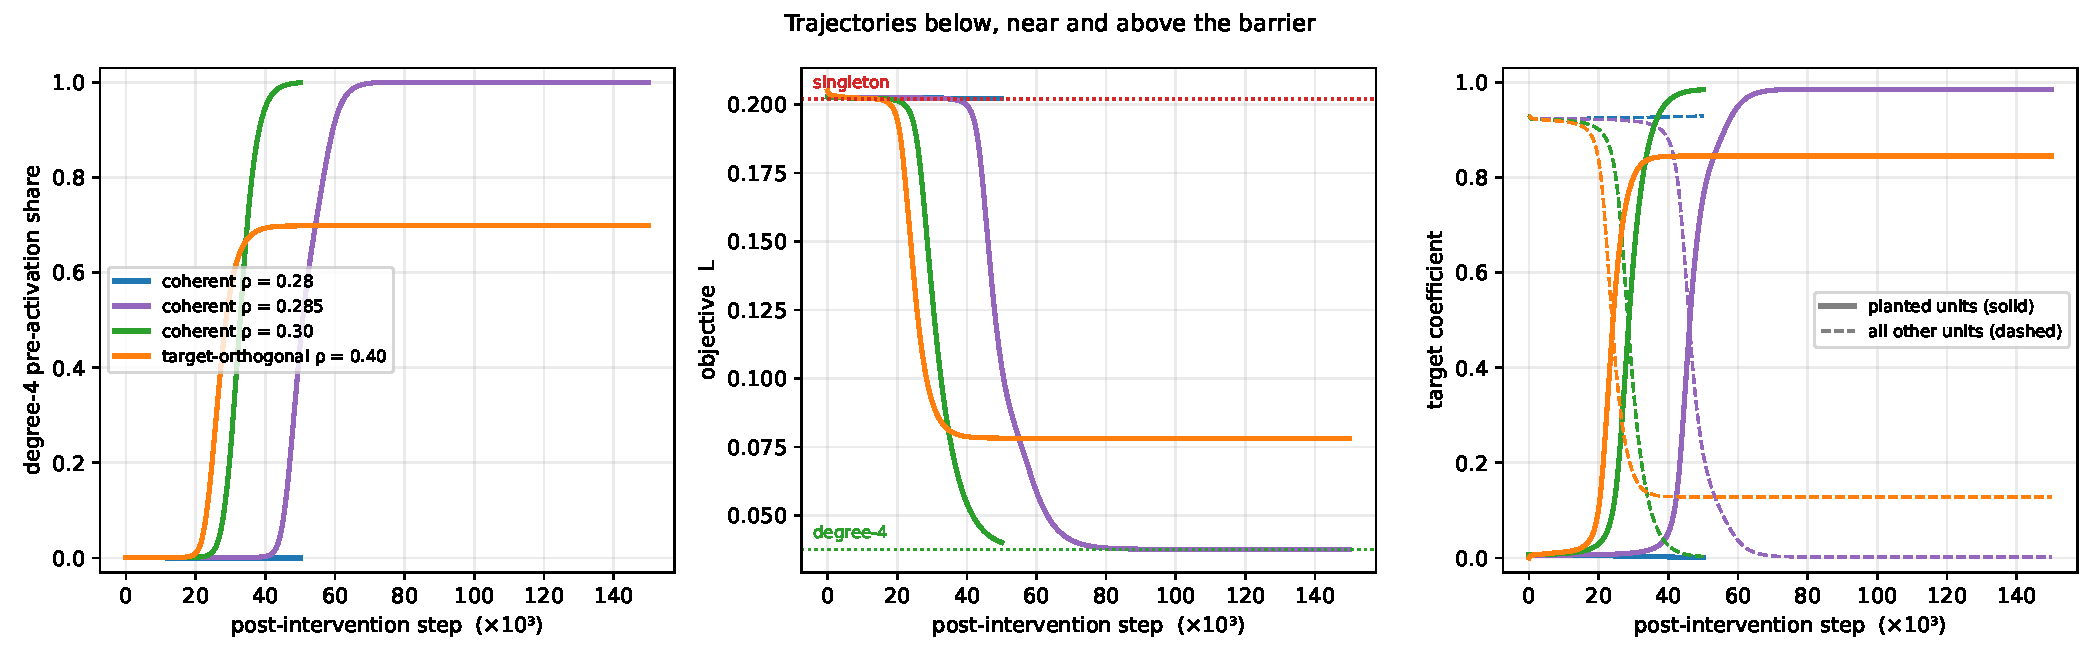
\includegraphics[width=0.95\textwidth]{rank1_bottleneck/plantd4_Q8_traj.pdf}\vspace{-4pt}
\caption{Trajectories below ($\rho=0.28$), just above ($0.285$, continued to 150k) and above ($0.30$) the
barrier, and the target-orthogonal control at $\rho=0.40$. Left: degree-4 share; middle: objective;
right: target coefficient carried by the four planted units (solid) and by all other units (dashed).}
\label{fig:traj}
\end{figure}


\textbf{3. The barrier is a basin boundary and the symmetric scalar description holds along the way.}
The initial projected gradient $2e\kappa_2\rho^2-\lambda\rho$ is negative up to $\rho\approx0.31$
($e=1-a\approx0.065$), so supercritical seeds first grow only through the slow decline of the incumbent:
at $\rho=0.285$ the templates reach $b=w=r=0.32$ only after 25k steps, then run away to $1.57$. Throughout,
$b,w,r$ stay equal to $0.3\%$ and the planted units' target coefficient equals $\tfrac14 bwr$ to better than
$10^{-4}$ until the takeover is nearly complete (final discrepancy $\le8\cdot10^{-3}$); singleton leakage into
the planted units stays below $10^{-6}$. Subcritical seeds shrink along all three templates together
($0.28\to0.135$ at 50k, accelerating).

\textbf{4. Target-orthogonal controls are not inert, and they are where the approximation fails.} At
$\rho=0.28$ and $0.34$ the planted units are overtaken by singleton leakage (leak fraction $0.93$ at 10k)
and the seed dies. At $\rho=0.40$ a coherent readout emerges from zero ($r_\parallel$ reaches $0.95$ by
30k) and a degree-4 circuit forms, but the network settles into a \emph{persistent mixed solution}: share
$0.70$, $\mathcal L=0.078$, planted coefficient $0.845$ and rest $0.129$, unchanged between 50k and 150k.
There the planted coefficient exceeds $\tfrac14 bwr$ by $0.64$, i.e.\ the circuit that forms is not the
symmetric template, and the ablations show both input families are needed (MSE $0.75$ with degree-4
only). At $\rho=0.60$ and $1.0$ the orthogonal controls are fully rescued ($\mathcal L=0.0377$, share $1$) but by a different route: the planted units carry only $0.73$ of the target and other units $0.25$--$0.26$, i.e.\ the degree-4 circuit recruits beyond the planted set, whereas every coherent seed ends with the planted four carrying $\ge0.985$.

\textbf{Answer.} The finite-seed barrier is observed; its location agrees with the reduced-model prediction
to within the grid spacing ($0.280<\rho_{\rm crit}<0.285$ vs.\ $0.2831$); the only deviations from the
scalar picture (mixed, asymmetric circuits) occur in the target-orthogonal controls, exactly where the
symmetric-circuit approximation does not apply.

\vspace{2pt}\footnotesize\sloppy
Code: \texttt{experiments/rank1\_bottleneck/plant\_degree4.py}, \texttt{plot\_plant\_degree4.py}, \texttt{tests/test\_plant\_degree4.py}. All arms: \texttt{reports/rank1\_bottleneck/plantd4\_Q8\_summary.csv}; per-arm \texttt{analysis/} folders in \texttt{analysis\_output/plantd4\_Q8/}; checkpoints on the training boxes (Drive prefixes \texttt{runs\_swish}, \texttt{runs\_germany2}).
\end{document}
